\documentclass[a4paper,12pt,twoside,english,openany]{book}
\usepackage[icon=Note,color=yellow,author=Sepand]{pdfcomment}
\usepackage[utf8]{inputenc}
\usepackage[figuresright]{rotating}
\usepackage[T1]{fontenc}
\usepackage{babel}
\usepackage[a4paper,left=3cm,right=2.5cm,top=3cm,bottom=3cm, twoside]{geometry}
\usepackage{xcolor}
\usepackage{stmaryrd}
\usepackage{amssymb}
\usepackage{amsmath}
\usepackage{libertine}
\usepackage[
    natbib=true,
    style=numeric,
    sorting=none,
    maxcitenames=1,
]{biblatex}

\addbibresource{res/biblio.bib} 
\addbibresource{res/biblio2.bib} 

\usepackage[font=small,labelfont=bf]{caption}
\usepackage{subcaption}
\usepackage{float}
\usepackage{multirow}
\usepackage[Export]{adjustbox}
\usepackage{array, multirow, tabularx}
\usepackage{booktabs}
\usepackage{longtable}
\usepackage{setspace}
\usepackage{apalike}
\usepackage{minitoc}
\usepackage{tikz}
\usetikzlibrary{calc, positioning, arrows.meta,arrows, shapes.geometric,backgrounds}
\usepackage[strict]{changepage}
\usepackage{siunitx}
\usepackage{enumitem}
\usepackage{epigraph}
\usepackage{lscape}
\usepackage{titletoc}
\usepackage{mdframed}
\usepackage{tabu}
\usepackage{pdfpages}
\usepackage{arydshln}
\usepackage{titling}
\usepackage{calc}
\usepackage[xindy]{imakeidx}
\usepackage{upgreek}
\usepackage{titlesec} 
\usepackage{sectsty}
\usepackage{lipsum}
\usepackage{emptypage}
\usepackage{fancyhdr}
\pagestyle{fancy}
\usepackage{graphicx}
\graphicspath{ {res/} }
\usepackage{hyperref} 
\hypersetup{
    colorlinks=true,
    linkcolor=black,
    filecolor=black,      
    urlcolor=black,
    citecolor=black,
    }
\definecolor{linkColor}{HTML}{32a852}

\titleformat{\chapter}[hang]
  {\normalfont\bfseries}{}{0pt}{\Huge}

\makeatletter
\renewcommand\section{%
  \@startsection{section}{1}{\z@}
  {1.5ex plus .2ex minus .2ex}
  {0.6ex}%                      
  {\normalfont\Large\bfseries}}

\renewcommand\subsection{%
  \@startsection{subsection}{2}{\z@}%
  {1.2ex plus .2ex minus .2ex}% before-skip
  {0.5ex}% after-skip
  {\normalfont\large\bfseries}}
\makeatother

\title{Estimation of Image-Derived Arterial Input Function in Brain PET Imaging: \\ Application to Modeling PET Dynamics of Glucose Metabolism in Patients with Impaired Consciousness}

\author{Sepand Ali Madad Soltani}
\date{March 2025}



\leftmark 
\rightmark 


% \makeindex
%\input{auxilliaires/glossaire}
\def\mrglu{\text{MR}_{\text{glu}}}
\newcommand{\fdg}{$[^{18}\mathrm{F}]\text{FDG}$}
\newcommand{\yohimbine}{$[^{11}\mathrm{C}]\text{Yohimbine}$}
\newcommand{\sym}[1]{\textsuperscript{#1}}


\begin{document}

\begin{titlepage}
	\begin{center}
		\begin{tabular}{c@{\hskip 7cm}c@{\hskip 1cm}}
			\includegraphics[height=3cm]{res/ucbl.png} &
			\includegraphics[height=3cm]{res/polytech2.png}
			% \includegraphics[width=5cm]{res/cermep.png}
		\end{tabular}
	\end{center}

	\begin{center}

		\vspace*{.03\textheight}
		\textsc{\Large University of Claude Bernard Lyon 1}\\[0.2cm]
		\large Polytech Lyon

		\rule{\textwidth}{0.8pt} \\
		\vspace{10pt}

		{\huge \bfseries \thetitle}
		\rule{\textwidth}{0.8pt} \\

		\vfill

		\vspace{18mm}

		{\Large \textsc{Sepand Ali Madad Soltani}}\\[3mm]
		{\large Master 2 in Medical Device Engineering}\\[1mm]
		{\large Internship Report}

		\vspace{12mm}

		{\normalsize \textit{Supervised by} \textsc{Inés Merida} \textit{and} \textsc{Nicolas Costes}}\\[2mm]
		{\normalsize \textit{Academic Advisor} \textsc{Kevin Tse-Ve-Koon}}

		\vspace{10mm}

		{\normalsize \textit{Hosting Laboratory}}\\
		{\normalsize CERMEP- imagrie du vivant, Bron, France}

		\vfill

		{\large 2024--2025}
		%
		%
		% \vfill
		% By \textsc{\Large Sepand Ali Madad Soltani}\\
		% Master 2 in Medical Device Engineering \\
		% Internship Report\\
		% Supervised by \textsc{\large Inés Mérida} and \textsc{\large Nicolas Costes}  \\
		% Academic Advisor: \textsc{\large Kevin Tse Ve Koon}\\
		% Hosting Laboratory:\\
		% CERMEP - Imagrie du Vivant, Lyon, France\\
		% 2024-2025
		%
	\end{center}

	\vspace{1cm}
\end{titlepage}

\renewcommand{\chaptermark}[1]{\markboth{#1}{}}


\frontmatter
\chapter*{Abstract}
\addcontentsline{toc}{chapter}{Abstract}

[TODO] 

\paragraph{Keywords:} Dynamic FDG-PET, Image-Derived Input Function, Hybrid PET/MRI, Bayesian Framework


\tableofcontents

\mainmatter
\setlength{\parskip}{.7em}

\renewcommand{\baselinestretch}{1.1}


\fancyhead[]{}
\fancyfoot[]{}
\fancyhead[LH]{\leftmark}
\fancyhead[RH]{\thepage}


\chapter{Introduction}
\section{Positron Emission Tomography}
Positron Emission Tomography (PET) is an in vivo functional imaging technique widely used in clinical and research settings to monitor physiological and biochemical processes.
In PET, a biologically active molecule is labeled with a positron-emitting radioisotope, serving as a radiotracer, and then injected into the body.
As the radiotracer accumulates in target tissues, its radioactive decay produces positrons, which interact with electrons to emit pairs of gamma photons in nearly opposite directions.
These photons are detected by the PET scanner, and image reconstruction algorithms generate a three-dimensional representation of the tracer distribution.
This imaging modality allows for the investigation of metabolic changes, receptor binding, and other biochemical processes, providing invaluable information in oncology, neurology, cardiology, and other fields.

There are two main categories in PET image acquisition: static imaging and dynamic imaging.
Static PET involves acquiring a single scan after the radiotracer injection.
This single snapshot offers a powerful yet simplified view of tracer distribution.
The common quantification metric in static imaging is the Standardized Uptake Value (SUV), which normalizes tissue uptake by the injected dose and weight of the subject, allowing for a semi-quantitative comparison of tracer accumulation across different tissues or over time \cite{keyes1995suv}.
Due to its simplicity, static PET is widely used in clinical settings; however, it also has limitations.
Because it reflects only one time point, the SUV cannot capture the temporal dynamics of tracer uptake and clearance, and various physiological factors may influence its measurements, thereby reducing its accuracy.

Dynamic PET imaging provides a more comprehensive view of radiotracer kinetics by acquiring a series of images over a period ranging from a few minutes to more than an hour post-injection, depending on the tracer type.
Instead of a single snapshot, dynamic imaging produces time-activity curves (TACs) that illustrate how tracer concentration in each tissue changes throughout the scanning period.
This approach enables the measurement of physiological parameters such as the tracer rate of influx (\(K_i\)) for radiotracers with irreversible uptake (e.g. \fdg ), volume of distribution (\(V_T\)), and the rates of phosphorylation and dephosphorylation.

\section{Kinetic Modeling}
To quantify pharmacokinetic parameters, kinetic modeling is employed.
Compartmental modeling is the most popular and is considered the most accurate approach in kinetic modeling.
In compartmental modeling, the distribution and kinetics of a radiotracer are described by dividing the system into distinct compartments, each representing a pool of tracer that behaves uniformly.
Interactions between compartments can be unidirectional or bidirectional, meaning the tracer may either move in and out or only enter a compartment.
Various graphical models (e.g., the Logan \cite{logan1990graphical} and Patlak \cite{patlak1983graphical} methods), as well as classical compartmental model fitting approaches, are used to analyze tracer kinetics.

Figure~\ref{fig:2tcm} shows the two-tissue compartment model (2TCM), also known as the three-compartment model, in series mode.
This model comprises one tissue compartment for the free tracer, \(C_F(t)\), and another for the receptor-bound tracer, \(C_B(t)\), in addition to an external compartment representing the tracer concentration in the plasma or blood, denoted as the input function \(C_P(t)\).

The tracer kinetics are governed by a series of first-order differential equations, in which the exchange rates between the compartments are considered constant:
\begin{align}
	\frac{dC_F(t)}{dt} & = K_1 \, C_P(t) \;-\; \bigl(k_2 + k_3\bigr) C_F(t) \;+\; k_4 C_B(t) \,, \label{eq:2tcm-c1} \\[6pt]
	\frac{dC_B(t)}{dt} & = k_3 \, C_F(t) \;-\; k_4 \, C_B(t), \label{eq:2tcm-c2}
\end{align}
where \(K_1\), \(k_2\), \(k_3\), and \(k_4\) are the constant rate parameters.

\begin{figure}[b]
	\centering
	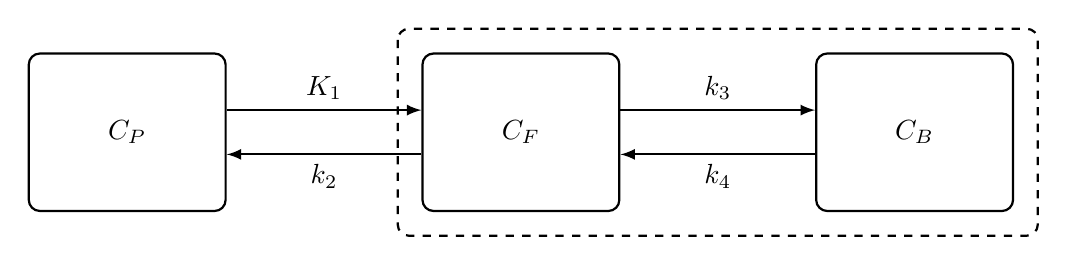
\begin{tikzpicture}[>=latex, thick]
		\node[draw, rounded corners, minimum width=2.5cm, minimum height=2cm, align=center] (Cp) at (0,0) {$C_P$};
		\node[draw, rounded corners, minimum width=2.5cm, minimum height=2cm, align=center] (C1) at (5,0) {$C_F$};
		\node[draw, rounded corners, minimum width=2.5cm, minimum height=2cm, align=center] (C2) at (10,0) {$C_B$};

		\draw[->]
		([yshift=8pt]Cp.east) to[out=0, in=180]
		node[above] {\(K_1\)}
		([yshift=8pt]C1.west);

		\draw[->]
		([yshift=-8pt]C1.west) to[out=180, in=0]
		node[below] {\(k_2\)}
		([yshift=-8pt]Cp.east);

		\draw[->]
		([yshift=8pt]C1.east) to[out=0, in=180]
		node[above] {\(k_3\)}
		([yshift=8pt]C2.west);

		\draw[->]
		([yshift=-8pt]C2.west) to[out=180, in=0]
		node[below] {\(k_4\)}
		([yshift=-8pt]C1.east);

		\draw[dashed, rounded corners, thick] ($(C1.north west)+(-0.3,0.3)$) rectangle ($(C2.south east)+(0.3,-0.3)$);

	\end{tikzpicture}
	\caption{Schematic of the two-tissue compartment model (2TCM)}
	\label{fig:2tcm}
\end{figure}

The total radiotracer tissular kinetic measured by PET (the PET data), \(C_T(t)\), is given by
\begin{equation}
	C_T(t) \;=\; C_F(t) \;+\; C_B(t) \;+\; C_P(t).
\end{equation}

Thus to solve this system of equations and to estimate \(K_1\), \(k_2\), and \(k_3\) parameters, we must fit the model using the measured PET TACs ($C_T$) and the input function ($C_P$).

For \fdg$\,$ quantification, the metabolic rate of glucose (\(\textrm{MR}_{\textrm{glu}}\)) is calculated as
\begin{equation}
	\textrm{MR}_{\textrm{glu}} \; (\textrm{\textmu mol/min/100g}) = \frac{[C]}{LC} \cdot \frac{K_1 \times k_3}{k_2 + k_3} \,.
\end{equation}
where \([C]\) denotes the glucose concentration, and \(LC\) is the lumped constant.

For \yohimbine $\,$ quantification, we utilize the Volume of Distribution ($V_T$) which is the ratio of radiotracer concentration in the target tissue ($C_T$) to the plasma ($C_P$):
\[
	V_T = \frac{C_T}{C_P}
\]

Using the Logan plot method this can be directly estimated from these two values or to be fitted to a compartment model. In the latter case, $V_T$ can be calculated as
\[
	V_T = \frac{K_1}{k_2} (1+\frac{k_3}{k_4})
\]


\section{Input Function}
\subsection{Arterial Input Function}
% GPT: Dont change
The arterial input function (AIF) is considered the gold standard for obtaining the input function.
It is determined by inserting an arterial catheter into the patient and continuously drawing blood samples to measure the radiotracer concentration, thereby obtaining the blood activity curve used in the quantification model.
However, this procedure is invasive and can cause discomfort, potentially discouraging patients from undergoing future examinations.
Furthermore, this method is labor-intensive and requires trained personnel to manage both the subject and the measurement devices.

\subsection{Image Derived Input Function}
% GPT: Dont change
The image-derived input function (IDIF) has been proposed as a non-invasive alternative for obtaining the input function.
IDIF techniques typically involve identifying vascular structures or regions with high blood pool activity within the imaging field and extracting the input function directly from the PET images.
In brain PET imaging, the carotid arteries are the largest vessels present in the limited field of view (FOV) and have a diameter of approximately 5 mm, which is comparable to the typical spatial resolution of PET (4-6mm FWHM).
Therefore, directly extracting the carotids from PET images is challenging due to the limited resolution and the strong partial volume effects (PVE) present.

\subsection{Population-Based Input Function}
Population-Based Input Function (PBIF) is a method for replacing the subject specifc AIF with the average AIFs of a population of other subjects.
% GPT: explain a bit more, max 1-2 sentences

\subsection{Background}
Many methods have utilized the first few frames of the dynamic PET where tracer only exists in the arteries and has not reached other tissues yet, to perform a high intensity tresholding to obtain the mask of the carotids \cite{young2023image}.
Due to PVE, these methods are not totally accurate therefore many different take clever approaches such as supervised clustering \cite{TODO}, Deep learning approaches \cite{TODO} and [TODO] \ref{TODO}



With the emergence of hybrid PET/MRI machines, it has become feasible to acquire both functional and anatomical data simultaneously.
MRI provides high-resolution soft tissue contrast, while PET captures metabolic activity.
For instance, time-of-flight MR angiography (TOF-MRA) delivers excellent arterial contrast, which allows for accurate segmentation of vascular structures such as the carotid arteries.
However, even with a high-resolution anatomical guidance, directly applying the segmented arterial mask to the PET images introduces challenges \cite{zanotti2011image}.
In particular, the limited spatial resolution of PET can lead to partial volume effects, resulting in inaccuracies in the derived input function.
Consequently, additional correction techniques are required to mitigate these effects and ensure reliable quantification.

Several methods have been developed to enhance IDIF accuracy by addressing partial volume correction and artery segmentation.
PET-only methods aim to extract the artery from the PET image itself which is


Several methods have been developed to enhance IDIF accuracy by addressing partial volume correction and automation challenges.
For partial volume correction,
Early PET-only approaches primarily focused on classical partial volume correction (PVC) techniques \cite{mourik2009image}, while more recent methods have explored supervised clustering algorithms \cite{lyoo2014image} and deep learning approaches \cite{chavan2024end,ferrante2024physically}.
Hybrid PET/MRI methods improve carotid artery delineation by leveraging anatomical imaging. The caliPER software, for instance, employs a semi-automated approach for IDIF extraction using carotid masks obtained from T1 or TOF-MRA images, incorporating partial volume correction \cite{dassanayake2022caliper}.
Additionally, fully automated methods have been proposed to enhance carotid segmentation and PVC techniques \cite{sari2017estimation, jochimsen2016fully, khalighi2018image, sundar2019towards}.

\citeauthor{irace2021bayesian} \cite{irace2021bayesian} proposed an automatique method for IDIF estimation by performing TOF-MRA driven carotid segmentation and using a Bayesian framework for incorporating prior knowledge into a geometric transfer matrix method \cite{rousset1998correction}---a classical partial volume correction technique.
In this work, the aim was to improve this method and enhance accuracy by evaluating it on a dataset of comatose patients.

\chapter{Materials and Methods}

\section{Dataset Description}
Two experimental dataset were available.
In the first study, 59 acute comatose patients were included between 7 days and 30 days after the coma onset (46 ± 16 years old; 21 females).
PET data were acquired in list mode during 90 min from the injection of an intravenous bolus of \fdg.
The second study, included 7 healthy subjects (25 ± 3 years old; all male) with injection of an intravenous bolus of \yohimbine.

Both dataset used the same exact following imaging protocol.
Simultaneously, an arterial time-of-flight MR (TOF-MRA)  in axial orientation, with a voxel size of 0.3$\times$0.3$\times$0.7 mm as well as a T1-weighted MRI in axial orientation, with isometric voxel size of 1mm were acquired.
Raw PET data were rebinned into 24-time frames (variable length frames : 8$\times$15 s, 3$\times$60 s, 5$\times$120 s, 1$\times$300 s, 7$\times$600 s) sinograms for dynamic reconstruction.
Reconstruction yielded a voxel size of 1.04$\times$1.04$\times$2.08 mm$^3$ in a matrix of 344$\times$344$\times$127 voxels.

In the \fdg  $\,$ study, AIF in the whole blood and plasma were measured from 26 arterial blood samples manually collected (with the following timing: every 5 s for the first minute, every 15 s until second minute, and at times 3, 5, 10, 20, 30, 45, 60, 75, 80, 85 and 90 minutes post-injection) and counted with a gamma counter.

In the \yohimbine $\,$study, 25 arterial blood samples were manually collected (with the following timing: every 5 s for the first minute, every 10 s until second minute, and at times 5, 10, 30, 45, 60, and 90 minutes post-injection).
The blood samples were counted with a gamma counter and were centrifuged and the extracted plasma was counted again to calculate the plasma fraction [TODO correct this part]


\section{Pre-processing}
For both studies, the T1-weighted image was registered to both the average PET image and to the TOF-MRA image using a affine registration method.
The two resulting affine transformation matrices were then combined to register the TOF-MRA directly to the PET.
Even though in the \fdg study, the patients were completely unconscious and the PET and MRI images were acquired simultaneously in the same session, this was still done out of an abundance of caution.
The T1-weighted image was used as a medium since it has common spatial features with both the other two modalities and directly registering TOF-MRA to the PET would be impractical due to the low spatial resolution of the PET and the limited axial FOV of the TOF-MRA images.

\section{Carotid Segmentation\label{sec:carotid}}
Figure~\ref{fig:seg_pipeline} shows the complete pipeline for the carotid segmentation.
Since vessels appear as hypersignal in TOF-MRA, a high-intensity thresholding technique can be used to extract the arteries from the image.
However, other tissues such as  brain lesion ---which were very common in the comatose dataset--- and venous structures may also appear as hypersignal and can interfere with the selection.
To exclude them, in a reference image, a cuboid volume of interest (VOI) was defined where the carotid arteries are most likely to appear (Step I).
The threshold value was calculated as the 1\% percentile of all non-zero voxels in the image and then it was applied to only to the voxels inside the VOI (Step II).
A 3D connectivity constraint was employed to the remaining voxels to extract all fully connected volumes and among those, the top 2 biggest were consider as the left and right internal carotid artery and extracted(Step III).

The reference image used was the standard MNI152 atlas, which was padded by 50\% more voxels in the inferior direction of the brain (negative Z in voxel-space) since the original atlas excludes the area below the brain which is of the interest for us.

The TOF-MRA image was then registered to the reference image using an affine registration technique and the obtained affine matrix was used to register and then apply the VOI to the TOF-MRA.

\begin{figure}[h]
	\centering
	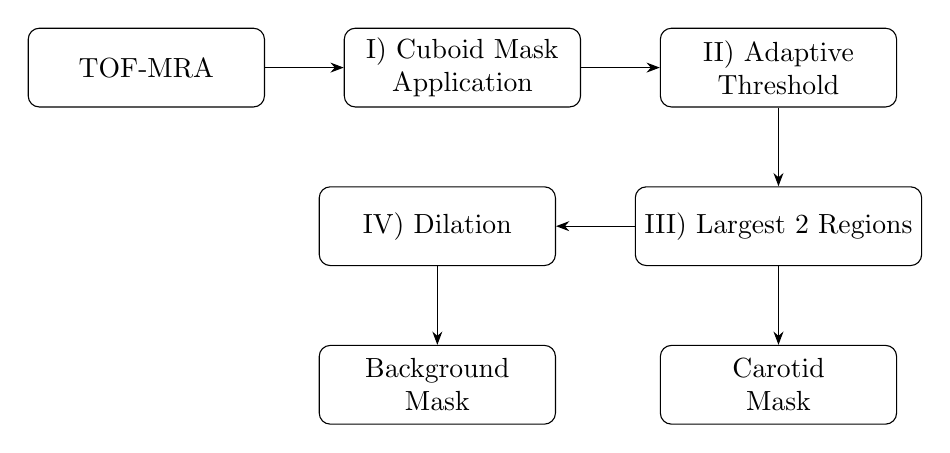
\begin{tikzpicture}[
			node distance=1cm,
			auto,
			>=Stealth,
			mybox/.style={draw, rounded corners, rectangle, minimum width=3cm, minimum height=1cm, align=center}
		]
		\node[mybox] (input) {TOF-MRA};
		\node[mybox, right=of input] (cuboid) {I) Cuboid Mask\\Application};

		\node[mybox, right=of cuboid] (thresh) {II) Adaptive\\ Threshold};
		\node[mybox, below=of thresh] (growing) {III) Largest 2 Regions};
		\node[mybox, left=of growing] (dilation) {IV) Dilation};
		\node[mybox, below=of growing] (mask) {Carotid\\Mask};
		\node[mybox, below=of dilation] (bg_mask) {Background\\Mask};

		\draw[->] (input) -- (cuboid);
		\draw[->] (cuboid) -- (thresh);
		\draw[->] (thresh) -- (growing);
		\draw[->] (growing) -- (mask);
		\draw[->] (growing) -- (dilation);
		\draw[->] (dilation) -- (bg_mask);
	\end{tikzpicture}
	\caption{Carotid and background mask segmentation pipeline}
	\label{fig:seg_pipeline}
\end{figure}

\section{Partial Volume Correction}
\subsection{Geometric Transfer Matrix}
As we discussed before in \ref{TODO}, direct extraction of the radioactivity in the arteries is not practical due to PVC.
Geometric Transfer Matrix aims to account for this loss of signal by considering the observed TACs are linear combination of the true value and other effecting regions \cite{rousset1998correction}.

Here we define two regions, the carotid and the surrounding tissues (background).
A mask for extracting the activities of the latter was obtained by dilating the carotid mask by 5 pixels and subtracting the voxels corresponding to the carotid mask (Figure~\ref{fig:seg_pipeline}, Step IV).

\begin{equation}
	\underbrace{
		\begin{bmatrix}
			T_{c} \\
			T_{bg}
		\end{bmatrix}
	}_{\text{Observed}}
	=
	\underbrace{
		\begin{bmatrix}
			\omega_{c \rightarrow c}  & \omega_{bg \rightarrow c}  \\
			\omega_{c \rightarrow bg} & \omega_{bg \rightarrow bg}
		\end{bmatrix}
	}_{\text{GTM}}
	.
	\underbrace{
		\begin{bmatrix}
			T_{IF} \\
			T_{tissue}
		\end{bmatrix}
	}_{\text{Unknown}},
\end{equation}

where $\omega_{n \rightarrow m}$ are the spill-in and spill-over coefficient of region $n$ onto region $m$, which is obtained by convolving the binary mask of region $n$ with the system's point spread function and integrating the resulting intensity over region $m$, normalized by the total signal in region $m$.
where
\begin{equation}
	\omega_{n\to m} = \frac{\displaystyle \int_{\Omega_m} \bigl( h \ast \chi_n \bigr)(r)\,dr}{\displaystyle \int_{\Omega_m} \bigl( h \ast \chi_m \bigr)(r)\,dr},
\end{equation}
with \(\chi_n\) and \(\chi_m\) denoting the binary masks of regions \(n\) and \(m\), respectively, \(h\) the system's point spread function, and \(\Omega_m\) the spatial domain of region \(m\).

$T_{c}$ and $T_{bg}$ are respectively the observed carotid and background TACs and $T_{IF}$ and $T_{tissue}$ are the real unknown TACs of the carotid (the input function) and the background tissue.

By inverting the GTM, this system of equations can be easily solved and the "true" TAC in the artery and background be computed.
% However, through a combination of small size of the carotids and short time frames and exponential decay of the tracer
However, GTM along with other classical PVE methods usually fail to fully recover the lost signal as they are a simplification that does not consider the whole picture particularly accounting for the time-variant noise experienced in the signal.
This causes these methods to not only fail to correct the noise but end up amplifying them because of their assumptions.
The time-variant noise can be attributed to number of contributing factors, namely, the small size of the arteries, very short frame-times at the beginning of the scan where the changes in the input function are very rapid and rapid decay of the radiotracer which in all result in low-count statistic hence having higher noise.

However, the GTM being a low rank matrix makes the inversion sensitive to noise and biased on small regions such as the carotid \cite{zanotti2011image, boellaard2004effects}.

\subsection{Bayesian Geometric Transfer Matrix}
\subsubsection{Modelling}
% To overcome challenges posed to GTM method, we utilized a Bayesian framework that jointly estimates the input function, the tissue activity and the system noise\cite{irace2021bayesian}.
For each subject, $T_{IF}$ is modeled as a linear combination of a population mean and its principal components.
These components are derived by performing principal component analysis (PCA) on a set of arterial input functions (AIFs) collected from the population.
Specifically, for each subject, a subset of 20 random subjects is selected from the dataset—excluding the subject under study—to construct the PCA model.
The data are first zero-centered, and PCA is applied to extract the principal axes \(\phi_i(t)\) and their corresponding explained variances \(\lambda_i\).
Each axis is then scaled by \(\sqrt{\lambda_i}\) to yield components \(v_i(t)\) with distribution of \(\mathcal{N}(0,1)\). The input function is then modeled as:

\begin{equation}
	T_{IF}(t) = \mu(t) + \sum_{i=1}^p \theta_i\,v_i(t),
\end{equation}

with
\[
	v_i(t) = \sqrt{\lambda_i}\,\phi_i(t),
\]
where $p$ is the number of components, \(\mu(t)\) is the population mean AIF, \(\phi_i(t)\) are the principal axes obtained from PCA, \(\lambda_i\) are their explained variances, and \(v_i(t)\) are the scaled components. Due to this scaling, the weighting coefficients \(\theta_i\) will have a distribution of \(\sim \mathcal{N}(0,1)\).

Spectral Analysis (SA) has been proposed as a decomposition method for describing the tissue activity in dynamic PET.
This method produces a spectrum of kinetic components by modelling the TACs as a convolution of the input function with a impulse response function \cite{TODO}.

The impulse response function is considered as sum of multiple exponentials. Therefor the background TAC will be
\[
	T_{bg} = \sum_{i=1}^s \alpha_{i} \cdot T_{IF} \circledast e^{-\beta_{i} t}.
\]
Where $\circledast$ denotes the convolution operator, \(\alpha_i\) is the coefficient. and \(\beta_i\) is the frequency of the \(i\)th spectrum.

In model fitting using SA, an appropriate spectral range is chosen based on the radioisotope half-life and is then divided in to $s=100$ or $s=1000$ fixed frequencies ($\beta$).
The distinct peaks in the resulting spectrum are kept.
In our model ,t his approach would not be efficient. Instead we select the number of spectral peaks and let the model to tune the frequencies and the amplitudes (see section \ref{TODO}).

\subsubsection{Noise}

Accurately modelling the noise is nearly impossible as there are numerous sources of them.
Some sources of noise such as scattering effect, random events, and motion artifacts among others are corrected to some degree by the reconstruction program.
However the biggest contributor of noise is "low-count statistics" which is caused by short time frames at the begin of the scan and by the exponential decay of the radioisotope towards the end of the scan apparent by the low dose of the tracer injection.
This combined with the small size of the carotid introduces a massive challenge for recovering the lost signal.

Noise in raw PET counts is considered to be a Poisson distribution however after the reconstruction process it is widely assumed to be a Gaussian distribution \cite{TODO}. To account for the previously mentioned time-variant noise, weights are used to normalize the noise along all frames to a single statistic. We define the weights as
\[
	\omega_{i} = \frac{\Delta t_i}{c_i} e^{\frac{-t_{i} ln(2)}{T_{1/2}}}
\]
where \(\omega_i\) is the weight, \(\Delta t_i\) is the frame duration, and \(c_i\) is the net-true counts detected by the PET camera at the \(i\)th frame and  \(T_{1/2}\) is the half-life of the radioisotope.
However, \(c_i\) was substituted here with \(C_T(t_i)\), the total radioactivity concentration at the mid-time frame due to unavailability of these counts in our dataset.

The time-variant noise variances can be normalized as the weighted mean of the per frame variance.

\[
	\sigma^2= \frac{1}{N} \sum_{i=1}^{N} \omega_i \sigma_i^2.
\]


\subsubsection{Estimation}
Let us define  \(\mathcal{D}\) as the observed PET TAC, \( \Theta = (\theta_{1}, \dots,\theta_{p}, \alpha_{1}, \beta_{1}, \dots, \alpha_{s}, \beta_{s}) \) as the set of unknown parameters describing the system, and consider an unknown Gaussian noise present in the system. We seek to estimate the joint probability \(p(\Theta,\sigma^2\mid \mathcal{D})\) of the model parameters \(\Theta\) and noise level given the observed data \(\mathcal{D}\)

According to the Bayes rule:
\[
	p(\Theta,\sigma^2 \mid \mathcal{D}) \propto p(\mathcal{D} \mid \Theta,\sigma^2) \cdot \pi( \Theta ) \cdot \pi( \sigma^2)
\]
where  \(p(\Theta,\sigma^2 \mid \mathcal{D})\) is the posterior distribution, \(p(\mathcal{D} \mid \Theta,\sigma^2)\) is the likelihood, and $\pi(\Theta)$ and $\pi(\sigma^2)$ are the prior knowledge that we have on the set of parameters and the noise. Thus we can sample the posterior distribution by calculate the likelihood and having the priors.


We can derive the observed data from the GTM response of the model \ref{TODO}. For convenience, we define
\[
	\mathcal{T}(t) = \mathcal{G}(t;\Theta) =
	\mathcal{G}\left(
	\begin{bmatrix}
			T_{IF}(t;\theta_{1}, \dots, \theta_{p}) \\
			T_{tissue}(t;\alpha_{1}, \beta_{1}, \dots)
		\end{bmatrix}\right)
\]
where $\mathcal{G}$ is the GTM model and $\mathcal{T}$ is the perceived activity based on the GTM model (effected by PVE). Since we considered the noise to be Gaussian, the likelihood would be

\[
	p(\mathcal{D} \mid \Theta,\sigma^2) = \prod_{i=1}^N \frac{1}{\sqrt{2\pi \sigma^2}} \exp\left( -\frac{\omega_i(\mathcal{D}(t_i) - \mathcal{T}(t_i))^2}{2\sigma^2} \right).
\]

The prior of parameters can be expanded as

\[
	\pi(\Theta) = \prod_{i=1}^p \pi(\theta_i)  \prod_{j=1}^s \pi(\alpha_j) \pi(\beta_j).
\]
As mentioned before, the PCA weighting coefficients have a normal distribution of $\mathcal{N}(0,1)$ which is also used as their prior knowledge.
The prior for the frequency and amplitude in SA was chosen as a reasonable uniform distribution range.
\[
	\alpha_i,\beta_i \sim \mathcal{U}( u_{\text{min}} , u_{\text{max}} )
\]

The prior distribution for the noise variance, $\pi(\sigma^2)$, is specified as an inverse-gamma distribution with hyperparameters $a_0$ and $b_0$ since inverse-gamma is the prior conjugate for the variance of a normal distribution
\[
	\sigma^2 \sim \Gamma^{-1}(a_0,b_0)
\]

In this work, the hyperparameters are selected so that $\pi(\sigma^2)$ is centered around an empirical estimate of the TAC variance, computed as the weighted root mean squared error between the observed carotid TAC and the mean AIF.

\[
	\mathbb{E}[X] = \frac{1}{N} \sum_{i=1}^{N} (T_c(t_i) - \mu(t_i))^2
\]
Thus by choosing a Coefficient of Variation (CV), we will have
\[
	a_0 = 2 + \frac{1}{\mathrm{CV}^2}\, , \, b_0 = (a_0 - 1) \, \mathbb{E}[X]
\]
\subsubsection{Sampling}

Evaluating the posterior distribution \ref{TODO} directly is not feasible due to its complexity and lack of a closed-form solution.
Thus we utilize a Monte-Carlo sampler to estimate the posterior distribution by taking sufficient random samples.
In this work, we utilize a Markov Chain Monte-Carlo with a hybrid Metropolis-within-Gibbs sampling method.

The Gibbs sampler allows for separately drawing sample for each parameter one by one based on its univariate posterior conditional distribution $p(\Theta_i \mid \mathcal{D}, \Theta_{-i}, \sigma^2)$ for each $\Theta_i$ where $\Theta_{-i}$ is the parameter vector except $\Theta_i$ and $p(\sigma^2 \mid \mathcal{D},\Theta)$ for the $\sigma^2$.

By iteratively doing this, Gibbs sampling results in the desired multivariate conditional posterior distribution $p(\Theta,\sigma^2 \mid \mathcal{D})$.

The exploration of the parameters $\Theta$ is done using the Metropolis-Hasting algorithm.
In this algorithm, a new parameter is proposed based on slightly changing the previous sample.
For example at the $m$th iteration in the chain, a new proposal for $\Theta_{i}^{(m)}$ is given as $\Theta_{i}^\prime = \Theta_{i}^{(m)} + \varepsilon_{i} \cdot b$, where $\varepsilon_{i}$ is the scaling factor or step-size and $b$ is a Brownian motion.
The proposal is either accepted and is kept as the new sample or rejected and the parameter stays unchanged.
The acceptance probability is given by
\[
	min\left(1,\frac{p(\Theta_i^\prime \mid \mathcal{D}, \Theta_{-i}, \sigma^2)}{p(\Theta_i^{(m)}\mid \mathcal{D}, \Theta_{-i}, \sigma^2)}\right)
\]

By choosing inverse-gamma for the noise prior which is conjugate prior, the posterior distribution is also a inverse-gamma distribution.

\[
	p(\sigma^2 \mid \mathcal{D},\Theta) \sim \Gamma^{-1}(a, b)
\]
where
\[
	a=a_0 + \frac{N}{2} \quad, b= b_0 + \sum_{i=0}^N \omega_i(\mathcal{D}(t_i) - \mathcal{T}(t_i))^2.
\]
Since we have a closed-form expression for the posterior distribution of the noise variance, we can just simply draw samples without the Metropolis-Hasting acceptance/rejection method.

To ensure efficient exploration of the parameter space, each parameter \( k \) is assigned its own proposal step size \( \epsilon_k \).
During the burn-in phase, these step sizes are adapted in blocks of \( L = 50 \) Metropolis–Hastings updates by monitoring the empirical acceptance rate for each parameter.
If the acceptance rate for a parameter exceeds 0.5, its step size is increased by an arbitrary 10\% (\( \epsilon_k \leftarrow 1.1\,\epsilon_k \)); otherwise, it is decreased by 10\% (\( \epsilon_k \leftarrow 0.9\,\epsilon_k \)).
This adaptive tuning continues until the end of the burn-in period, after which all step sizes are fixed and subsequent samples are retained.

\subsubsection{Inference}
After sufficient sampling, we employ a modified Maximum a Posteriori (MAP) method by calculating the average parameters of the top 0.1\% samples with the highest posterior probability and considering it as the solution.



\section{Evaluation}
\subsection{IF Curves}
The performance of the proposed IDIF estimation was first evaluated by computing the mean absolute error (MAE) between the cumulative area under the curve (cAUC) of the estimated IDIF and the \textit{ground true} AIF. cAUC was considered to be a more suitable metric since it provides an integrated measure of tracer exposure over time and is less sensitive to local fluctuations or noise in the curve compared to the directly comparing the TACs.
\begin{equation}
	\textrm{cAUC}(t) =  \int_{0}^{t} IF(\tau) \, d\tau,
\end{equation}
where \(IF\) is the input function.

\subsection{Quantification}
However, because the cAUC error does not fully capture the impact of IDIF deviations on kinetic parameters, absolute quantification was also performed to evaluate the performance of the estimated IDIF against the gold standard AIF.
This was achieved by utilizing an irreversible two-tissue compartment model (2TCM) via non-linear fitting with the \texttt{fitk3} program from the TPCCLIB library developed at the Turku PET Centre \cite{oikonen2018tpcclib}—applying the model fitting once with the IDIF and once with the AIF as the input function.

The brain was segmented into regions of interest (ROI) based on the Hammersmith brain atlas \cite{hammers2003three}, and TACs were generated by averaging voxels over each ROI at every time point.
The regional influx rate (\(K_i\)) was then calculated, from which the corresponding \(\mrglu\) values were derived.

The mean absolute percentage error (MAPE) of the \(\textrm{MR}_{glu}\) in each ROI was calculated and then averaged across the entire dataset:
\begin{equation}
	\text{Average MAPE}(\mrglu)= \frac{100\%}{N} \sum_{i=1}^{N} \left( \frac{1}{N_{\text{ROI}}} \sum_{j=1}^{N_{\text{ROI}}} \left| \frac{\textrm{MR}_{\textrm{glu},ij}^{\textrm{IDIF}} - \textrm{MR}_{\textrm{glu},ij}^{\textrm{AIF}}}{\textrm{MR}_{\textrm{glu},ij}^{\textrm{AIF}}} \right| \right),
\end{equation}
where $N$ is the number of subjects.

Additionally, linear least-squares regression was performed between the regional \(\mrglu\) obtained by quantification with using AIF and IDIF for each subject. The coefficient of determination (\(R^2\)) and the regression slope (\(S\)) were obtained for each subject. The mean absolute errors of these metrics across the dataset are given by
\begin{equation}
	\text{MAE}(R^2) = \frac{1}{N} \sum_{i=1}^{N} \left| R^2_i - 1 \right|
\end{equation}
and
\begin{equation}
	\text{MAE}(S) = \frac{1}{N} \sum_{i=1}^{N} \left| S_i - 1 \right|,
\end{equation}
where $N$ is the number of subjects and \(R^2_i\) and \(S_i\) denote the coefficient of determination and the regression slope for subject \(i\), respectively.

\section{Simulation}
PET simulations are an integral part of the validation of statistical and analytical PET methods as they have the advantage of knowing the exact ground truth which is not always available or might be effected by human or instrument malfunction.
In the previous section, we considered the AIF to be the gold standard and the ground truth and the evaluation was done by comparing the method to it.
But since the AIF is taken and analysed manually and involves multiple devices and processes operated by different personnels (nurses and chemists) at different steps, there is a large possibility for mistakes.

For this reason, as a complementary validation step to the experimental datasets, simulations were conducted and the method will be evaluated on them as well.

PET-SORTEO is a realistic Monte-Carlo PET simulation platform

\chapter{Results}
\section{Carotid Segmentation from MRA-TOF}
% GPT: fix sentencing 
As illustrated in Figure~\ref{fig:seg_compare}, the cuboid mask plays a crucial role in the carotid segmentation.
Because no ground truth segmentation is available, visual inspection was used to evaluate the results.
In Figure~\ref{TODO}, we see the 3D model of segmented ICA of a subject.

\begin{figure}[h]
	\centering
	\includegraphics[width=0.3\textwidth]{figures/carotid_3d.jpg}
	\caption{3D visualization of segmented internal carotid arteries}
\end{figure}

\begin{figure}[h]
	\centering
	\begin{subfigure}{0.45\textwidth}
		\includegraphics[width=\textwidth]{figures/molgu07704_bbox.png}
		\caption{}
		\label{subfig:seg_bbox}
	\end{subfigure}
	\begin{subfigure}{0.45\textwidth}
		\includegraphics[width=\textwidth]{figures/molgu07704_nobbox.png}
		\caption{}
		\label{subfig:seg_nobbox}
	\end{subfigure}
	\caption{Comparison of carotid segmentation (green) with (a) and without (b) a cuboid mask (yellow). In the absence of the cuboid mask, the segmentation algorithm fails to capture the carotid and instead incorrectly identifies the brain lesion}
	\label{fig:seg_compare}
\end{figure}


% GPT: Hyperparameter is the correct term?
\section{Hyperparameter Tuning}
% GPT: fix sentencing and coherence
The number of principle components $p$ was chosen as 3 by analysing the explained variance ratio plot in Figure~\ref{TODO}.
We see with only 3 components we get more than 90\% explained variability.
To prove the availability of the method, we seek to find the lowest possible number of population needed for the PCA in our \fdg $\,$ dataset.
To do this, the experiment was repeated 10 times each time with a different random seed for choosing population for $N=\{5,10,15,20,30,40,50,60\}$ and the median quantification errors were compared.
As apparent in Figure~\ref{TODO}, we see a plateau in the performance after $N=20$ and it was chosen as the ideal population sample count.
For the \yohimbine$\,$ dataset since it only has 7 subjects, the maximum amount $N=6$ was chosen.


\begin{figure}[h]
	\centering
	\includegraphics[width=\textwidth]{figures/pca_explained_variance.jpg}
	% gpt: add caption its the x=n components, y=cumulative explained variance % plot
	\caption{}
\end{figure}
\begin{figure}[h]
	\centering
	\includegraphics[width=0.8\textwidth]{figures/pca_n_experiment.jpg}
	%gpt: its the plt.xlabel("PCA population size (N)"); plt.ylabel("MAPE Quantification Error (median ± 95% CI)") errorplot
	\caption{}
\end{figure}

% GPT: fix sentencing and coherence
In classical model fitting using SA, an appropriate spectral range is chosen based on the radioisotope half-life (e.g. $10^{-4} \mathrm{s}^{-1}$ to $1 \mathrm{s}^{-1}$ for $^{18}\mathrm{F}$ ) and is then divided in to $s=100$ or $s=1000$ fixed frequencies ($\beta$) then their amplitudes ($\alpha$) are fitted to the TAC \cite{TODO}.
The peaks in the resulting spectrum are considered as the [TODO] frequencies of the TAC.
However, estimating 100 or 1000 different amplitude parameters using MCMC would not be computationally feasible.
Instead we must chose an appropriate number of spectral components and let the model to tune the frequencies and the amplitudes together.

To derive the number of basis functions, we assumed the activity in the surrounding tissue can either be modelled as 1TCM or 2TCM which their Impulse Response Function (IRF) have respectively one and two basis functions.
Experiments with two basis functions showed that the model rarely results in two distinctive frequencies and would generally converge to similar values for both frequencies or one frequency would converge to infinity meaning no signifiant impact.
Thus for both datasets one basis function was chosen.

As discussed in Section~\ref{TODO}, the prior distribution used for the PCA weighting coefficients was $\theta_i \sim \mathcal{N}(0,1)$.
The prior for the SA parameters were considered a very uninformative uniform distribution $\mathcal{U}(10^{-5},10^{-2})$ as we did not have concrete prior knowledge on these parameters.


\section{Simulation}
% GPT: fix sentencing and coherence
From the 59 subjects in the \fdg $\,$ dataset, 24 subjects were excluded due to having very large brain tumors or opened skulls due to open brain surgery which caused the tissue classification algorithm to fail.
The rest of the 35 subjects were used to create the numerical phantoms and to generate TACs for the simulation protocol.
PET-SORTEO utilized the protocols to simulate realistic PET kinetic and exported PETs in sinogram format.
The sinograms were reconstructed with the same reconstruction program and settings as the experimental dataset to ensure uniformity with the experimental dataset.

Although the point of the simulation was not to replicate the same scan exactly but only use it as an inspiration for how tracer kinetic behavior, the results of the simulations were compared to the real scans as a quality control step.
In Figure~\ref{TODO} we see an example of the 2nd (top) and last frame (bottom) sagittal slice of the real PET(inspiration source), the simulation input, and the simulation output from left to right.
As expected we see less details in the neck area (SOFT region) since we did not consider the complete arterial and venous structure as well as glands.
But more importantly, we can clearly see the activity in the internal carotids in the 2nd frame which roughly coincides with the peak of the AIF.
In the last frame we can also see the steady-state activity of the brain to be very realistic and have realistic contrast in different regions.

In Figure~\ref{TODO}, we see an example of the comparison of the Partial Volume Corrected TAC of the simulation output and the simulation input.
As expected we notice slight discrepancy due to lost signal as noise in the larger regions such as GM, CGM, and WGM since they are less affected by PVE and a very noticeable bias in the ICA which is affected the most by PVE.

As a post processing step, the brain atlases were also applied to the reconstructed simulated PETs to extract regional TTACs for the quantification step.

% gpt: make it in to figure and add appropriate caption:
\begin{figure}[h]
	\centering
	\includegraphics[width=\textwidth]{figures/sim_compare.jpg}
	\caption{}
\end{figure}

% gpt: make it in to figure and add appropriate caption ( its the comparison one)
\begin{figure}[h]
	\centering
	\includegraphics[width=0.4\textwidth]{figures/sim_tac.png}
	\caption{}
\end{figure}

\section{IDIF}

% GPT: fix sentencing and coherence
Since BGTM relies on the GTM method and also depends on a population AIF. Thus the performance should be compared compared to the IDIF derived from GTM method and also the Population Based Input Function (PBIF) which is the mean AIF used in the PCA (\(\mu_{IF}\)).
The Markov Chain was run for 230,000 iteration of which the first 30,000 were in the burn-in stage.

\subsection{\fdg\ Dataset}
% GPT: fix grammar issues and sentencing. don't change a lot
The reported statistic are from the experiment with the median results from the fine-tuning stage.

Figure~\ref{fig:fdg_ifs} compares the two methods for one of the best- and worst-performing subjects.
In the well-performing subject, BGTM significantly outperforms GTM and PBIF($\mrglu$ MAPE of 1.2\% vs. 26\% and 1.6\% respectively); however, in the poorly performing case, BGTM falls short of GTM and PBIF ($\mrglu$ MAPE of 36\% vs. 2.2\% and 4.75\% respectively).

\begin{figure}[h]
	\centering
	\begin{subfigure}[b]{0.322\textwidth}
		\includegraphics[width=\textwidth]{figures/PM10845_1_infunc.png}
		\caption{}
	\end{subfigure}
	\begin{subfigure}[b]{0.322\textwidth}
		\includegraphics[width=\textwidth]{figures/PM10845_1_cauc.png}
		\caption{}
	\end{subfigure}
	\begin{subfigure}[b]{0.322\textwidth}
		\includegraphics[width=\textwidth]{figures/PM10845_1_patlak_mrglu.png}
		\caption{}
	\end{subfigure}
	\begin{subfigure}[b]{0.322\textwidth}
		\includegraphics[width=\textwidth]{figures/COUJE07810_1_infunc.png}
		\caption{}
	\end{subfigure}
	\begin{subfigure}[b]{0.322\textwidth}
		\includegraphics[width=\textwidth]{figures/COUJE07810_1_cauc.png}
		\caption{}
	\end{subfigure}
	\begin{subfigure}[b]{0.322\textwidth}
		\includegraphics[width=\textwidth]{figures/COUJE07810_1_patlak_mrglu.png}
		\caption{}
	\end{subfigure}
	\caption{Comparison of the IFs (a,d), cumulative AUC curves (b,e), and $\mrglu$ regression lines (c,f) for one of the best-(top row) and worst-performing(bottom row) subjects in the \fdg\ dataset}
	\label{fig:fdg_ifs}
\end{figure}

The average mean absolute error of the cAUC curves across the dataset was 13,024 for BGTM and 15,709 and 14,630 for GTM and PBIF respectively (Figure~\ref{subfig:fdg_cauc_boxplot}).
In quantification BGTM resulted in better performance compared to GTM and PBIF methods.
Specifically, the BGTM, GTM, and PBIF methods achieved an average \(\mrglu\) mean absolute percentage error (MAPE) of 13\%, 24\%, 17\%, respectively (Figure~\ref{subfig:fdg_mape_boxplot}), and an average \(\mrglu\) MAE of 1.04, 1.98, and 1.4.
In addition, the MAPE for the coefficient of determination (\(R^2\)) and the regression slope (\(S\)) were 1.75\%, 11.2\% for BGTM, compared to 4.1\% and 17\% for GTM and 1.5\% and 15.75\% for PBIF, respectively.

\begin{figure}[h]
	\centering
	\begin{subfigure}[b]{0.45\textwidth}
		\includegraphics[width=\textwidth]{figures/fdg_quantification_patlak_mape_boxplot.png}
		\caption{\(\mrglu\) MAPE Boxplot}
		\label{subfig:fdg_mape_boxplot}
	\end{subfigure}
	\begin{subfigure}[b]{0.45\textwidth}
		\includegraphics[width=\textwidth]{figures/fdg_curve_mae_boxplot.png}
		\caption{cAUC MAE Boxplot}
		\label{subfig:fdg_cauc_boxplot}
	\end{subfigure}
	\caption{Boxplot of curve and quantification errors for the \fdg\ dataset}
	\label{fig:fdg_boxplots}
\end{figure}




% GPT: dont touch
Paired t-tests were used to compare BGTM with GTM and PBIF on quantification metrics (Table~\ref{tab:metrics_all_fdg}).
Relative to GTM, BGTM showed significantly lower \(\mrglu\) MAE (\(t=-5.934, p=1.754\times 10^{-7}\)), \(\mrglu\) MAPE (\(t=-5.459,\,p=1.042\times 10^{-6}\)), \(R^2\) absolute percentage error (APE) (\(t=-2.762,\,p=7.677\times 10^{-3}\)), and slope APE (\(t=-4.030,\,p=1.644\times 10^{-4}\)).
Relative to PBIF, BGTM also yielded significantly lower \(\mrglu\) MAE (\(t=-2.974,\,p=4.275\times 10^{-3}\)), \(\mrglu\) MAPE (\(t=-2.415,\,p=1.890\times 10^{-2}\)), and slope APE (\(t=-3.036,\,p=3.583\times 10^{-3}\)), while the difference in \(R^2\) APE was not significant (\(t=1.680,\,p=9.832\times 10^{-2}\)).


\subsection{\yohimbine\ Dataset}

% GPT: fix grammar sentencing and coherence. should i keep the "it's mostly a lucky exception" or move it to discussion?
The success of the \fdg\ dataset was not able to be replicated for the \yohimbine\ dataset.
In Figure~\ref{fig:yoh_ifs} the best- and worst-performing subjects are compared.
However, the 5\% MAPE $V_T$ in the good performing subject cannot reliably be attributed to the well performance of the algorithm rather it's mostly a lucky exception.

Overall the average cAUC MAE of the dataset was 55{,}499 for BGTM and 96{,}362 and 37{,}613 for GTM and PBIF, respectively (Figure~\ref{subfig:yoh_cauc_boxplot}).
In quantification using Logan plot method, the average \(V_T\) MAPE was 75.9\%, 166.5\%, and 29.5\% for BGTM, GTM, and PBIF, respectively (Figure~\ref{subfig:yoh_mape_boxplot}).

As apparent by the Paired t-tests in Table~\ref{tab:metrics_all_yoh}, BGTM was able to perform better than GTM but performs significantly worst than the PBIF method.

\begin{figure}[h]
	\centering
	\begin{subfigure}[b]{0.322\textwidth}
		\includegraphics[width=\textwidth]{figures/LUCAU08056_TEST_infunc.png}
		\caption{}
	\end{subfigure}
	\begin{subfigure}[b]{0.322\textwidth}
		\includegraphics[width=\textwidth]{figures/LUCAU08056_TEST_cauc.png}
		\caption{}
	\end{subfigure}
	\begin{subfigure}[b]{0.322\textwidth}
		\includegraphics[width=\textwidth]{figures/LUCAU08056_TEST_logan_bp.png}
		\caption{}
	\end{subfigure}
	\begin{subfigure}[b]{0.322\textwidth}
		\includegraphics[width=\textwidth]{figures/GOIAX07977_TEST_infunc.png}
		\caption{}
	\end{subfigure}
	\begin{subfigure}[b]{0.322\textwidth}
		\includegraphics[width=\textwidth]{figures/GOIAX07977_TEST_cauc.png}
		\caption{}
	\end{subfigure}
	\begin{subfigure}[b]{0.322\textwidth}
		\includegraphics[width=\textwidth]{figures/GOIAX07977_TEST_logan_bp.png}
		\caption{}
	\end{subfigure}
	\caption{Comparison of the IFs (a,d), cumulative AUC curves (b,e), and $V_T$ regression lines (c,f) for one of the best-(top row) and worst-performing(bottom row) subjects in the \yohimbine\ dataset}
	\label{fig:yoh_ifs}
\end{figure}

\begin{figure}[h]
	\centering
	\begin{subfigure}[b]{0.45\textwidth}
		\includegraphics[width=\textwidth]{figures/yoh_quantification_logan_mape_boxplot.png}
		\caption{\(\mrglu\) MAPE Boxplot}
		\label{subfig:yoh_mape_boxplot}
	\end{subfigure}
	\begin{subfigure}[b]{0.45\textwidth}
		\includegraphics[width=\textwidth]{figures/yoh_curve_mae_boxplot.png}
		\caption{cAUC MAE Boxplot}
		\label{subfig:yoh_cauc_boxplot}
	\end{subfigure}
	\caption{Boxplot of curve and quantification errors of the \yohimbine\ dataset}
	\label{fig:yoh_boxplots}
\end{figure}


\subsection{Simulated Dataset}
% GPT: fix sentencing
As a complementary quality control step of the simulations, the performance of Direct IDIF (meaning with no PVC) of the experimental dataset was compared to the simulated dataset.
The average cAUC MAE of the simulated dataset was significantly higher than the experimental dataset (85,138 vs 34,929).
And the AUC APE of 46\% for simulated compared to 22\% for experimental.
By comparing the temporal error of the Direct IDIF curves of both dataset (example subject in Figure~\ref{fig:sim_temporal_err}), it was shown that the Direct IDIF of the simulated data underestimates the activity level compared to the experimental data.

This underestimation and larger bias in the Direct IDIF was translated in to large bias in the other IDIF methods as well.
Figure~\ref{fig:sim_ifs} compares one of the best and worst-performing subjects.
BGTM was only able to show slight improvement in cAUC MAE compared to GTM with 53,997 vs 57,991.
However, it performed significantly worse than PBIF with an average bias of 23,072(Figure~\ref{subfig:sim_cauc_boxplot}.
In absolute quantification, BGTM underperformed compared to both methods with an average $\mrglu$ MAPE of 48\% compared to 35.6\% and 18.5\% for GTM and PBIF respectively.
In Table~\ref{tab:metrics_all_sim}, the performance in all metrics are detailed and no significant improvement was noticed in the paired t-tests.

\begin{figure}[h]
    \includegraphics[width=\textwidth]{figures/GM12051_temporal_error.png}
    \caption{Comparison of Relative Temporal Bias Percentage of the experimental and simulated data Direct IDIF of a subject}
    \label{fig:sim_temporal_err}
\end{figure}

\begin{figure}[h]
	\centering
	\begin{subfigure}[b]{0.322\textwidth}
		\includegraphics[width=\textwidth]{figures/sim_CHAAB07833_1_infunc.png}
		\caption{}
	\end{subfigure}
	\begin{subfigure}[b]{0.322\textwidth}
		\includegraphics[width=\textwidth]{figures/sim_CHAAB07833_1_cauc.png}
		\caption{}
	\end{subfigure}
	\begin{subfigure}[b]{0.322\textwidth}
		\includegraphics[width=\textwidth]{figures/sim_CHAAB07833_1_patlak_mrglu.png}
		\caption{}
	\end{subfigure}
	\begin{subfigure}[b]{0.322\textwidth}
		\includegraphics[width=\textwidth]{figures/sim_AJ10923_1_infunc.png}
		\caption{}
	\end{subfigure}
	\begin{subfigure}[b]{0.322\textwidth}
		\includegraphics[width=\textwidth]{figures/sim_AJ10923_1_cauc.png}
		\caption{}
	\end{subfigure}
	\begin{subfigure}[b]{0.322\textwidth}
		\includegraphics[width=\textwidth]{figures/sim_AJ10923_1_patlak_mrglu.png}
		\caption{}
	\end{subfigure}
	\caption{Comparison of the IFs (a,d), cumulative AUC curves (b,e), and $\mrglu$ regression lines (c,f) for one of the best-(top row) and worst-performing(bottom row) subjects in the simulated dataset}
	\label{fig:sim_ifs}
\end{figure}

\begin{figure}[h]
	\centering
	\begin{subfigure}[b]{0.45\textwidth}
		\includegraphics[width=\textwidth]{figures/sim_quantification_patlak_mape_boxplot.png}
		\caption{\(\mrglu\) MAPE Boxplot}
		\label{subfig:sim_mape_boxplot}
	\end{subfigure}
	\begin{subfigure}[b]{0.45\textwidth}
		\includegraphics[width=\textwidth]{figures/sim_curve_mae_boxplot.png}
		\caption{cAUC MAE Boxplot}
		\label{subfig:sim_cauc_boxplot}
	\end{subfigure}
	\caption{Boxplot of curve and quantification errors of the simulated dataset}
	\label{fig:sim_boxplots}
\end{figure}

% GPT: Don't touch tables
\begin{sidewaystable}[b]
	\centering
	\small
	\setlength{\tabcolsep}{10pt}
	\begin{tabular}{l|cc|cc|cc|cc|cc}
		\toprule
		\multirow{2}{*}{\textbf{Metric}} & \multicolumn{2}{c|}{\textbf{BGTM}} & \multicolumn{2}{c|}{\textbf{GTM}} & \multicolumn{2}{c|}{\textbf{PBIF}} & \multicolumn{2}{c|}{\textbf{BGTM vs GTM}} & \multicolumn{2}{c}{\textbf{BGTM vs PBIF}}                                                                                                                  \\
		\cmidrule(lr){2-3} \cmidrule(lr){4-5} \cmidrule(lr){6-7} \cmidrule(lr){8-9} \cmidrule(lr){10-11}
		                                 & \(\mu\)                            & \(\sigma\)                        & \(\mu\)                            & \(\sigma\)                                & \(\mu\)                                   & \(\sigma\) & \(t\)      & \(p\)                              & \(t\)      & \(p\)                              \\
		\midrule
		IF cAUC MAE                      & 13{,}024                           & 10{,}410                          & 15{,}709                           & 7{,}884                                   & 14{,}630                                  & 10{,}268   & \(-2.388\) & \(2.023\times 10^{-2}\) \sym{*}    & \(-1.278\) & \(2.065\times 10^{-1}\)            \\
		IF cAUC RMSE                     & 20{,}293                           & 16{,}078                          & 23{,}380                           & 11{,}979                                  & 23{,}334                                  & 16{,}803   & \(-1.907\) & \(6.151\times 10^{-2}\) \sym{\dag} & \(-1.439\) & \(1.555\times 10^{-1}\)            \\
		IF AUC APE (\%)                  & 11.93                              & 10.76                             & 11.57                              & 11.50                                     & 14.34                                     & 11.08      & \(0.297\)  & \(7.674\times 10^{-1}\)            & \(-1.862\) & \(6.767\times 10^{-2}\) \sym{\dag} \\
		\midrule
		\(\mrglu\) MAPE (\%)             & 13.19                              & 10.57                             & 24.36                              & 13.68                                     & 17.17                                     & 12.41      & \(-5.459\) & \(1.042\times 10^{-6}\) \sym{***}  & \(-2.415\) & \(1.890\times 10^{-2}\) \sym{*}    \\
		\(\mrglu\) MAE                   & 1.04                               & 0.92                              & 1.98                               & 1.33                                      & 1.40                                      & 1.10       & \(-5.934\) & \(1.754\times 10^{-7}\) \sym{***}  & \(-2.974\) & \(4.275\times 10^{-3}\) \sym{**}   \\
		\(R^2\) APE (\%)                 & 1.76                               & 4.07                              & 4.13                               & 8.90                                      & 1.50                                      & 3.53       & \(-2.762\) & \(7.677\times 10^{-3}\) \sym{**}   & \(1.680\)  & \(9.832\times 10^{-2}\)            \\
		Slope APE (\%)                   & 11.28                              & 9.37                              & 17.05                              & 10.58                                     & 15.76                                     & 11.41      & \(-4.030\) & \(1.644\times 10^{-4}\) \sym{***}  & \(-3.036\) & \(3.583\times 10^{-3}\) \sym{**}   \\
		\bottomrule
	\end{tabular}
	\caption{Comprehensive curve and quantification metrics for the \fdg\ dataset.
		Values are means (\(\mu\)) and standard deviations (\(\sigma\)) across subjects.
		Paired two-sided \(t\)-tests compare GTM or PBIF against BGTM for each metric.
		Significance codes: \sym{*}\,p<0.05, \sym{**}\,p<0.01, \sym{***}\,p<0.001, \sym{\dag}\,p<0.10 (trend).}

	\label{tab:metrics_all_fdg}
\end{sidewaystable}
\begin{sidewaystable}[b]
	\centering
	\small
	\setlength{\tabcolsep}{10pt}
	\begin{tabular}{l|cc|cc|cc|cc|cc}
		\toprule
		\multirow{2}{*}{\textbf{Metric}} & \multicolumn{2}{c|}{\textbf{BGTM}} & \multicolumn{2}{c|}{\textbf{GTM}} & \multicolumn{2}{c|}{\textbf{PBIF}} & \multicolumn{2}{c|}{\textbf{BGTM vs GTM}} & \multicolumn{2}{c}{\textbf{BGTM vs PBIF}}                                                                                                  \\
		\cmidrule(lr){2-3} \cmidrule(lr){4-5} \cmidrule(lr){6-7} \cmidrule(lr){8-9} \cmidrule(lr){10-11}
		                                 & \(\mu\)                            & \(\sigma\)                        & \(\mu\)                            & \(\sigma\)                                & \(\mu\)                                   & \(\sigma\) & \(t\)      & \(p\)                          & \(t\)      & \(p\)                  \\
		\midrule
		IF cAUC MAE                      & 55{,}499                           & 40{,}271                          & 96{,}362                           & 20{,}343                                  & 37{,}613                                  & 20{,}456   & \(-3.404\) & \(1.443\times10^{-2}\)\sym{*}  & \(0.959\)  & \(3.748\times10^{-1}\) \\
		IF cAUC RMSE                     & 83{,}282                           & 60{,}130                          & 147{,}032                          & 28{,}318                                  & 52{,}313                                  & 27{,}845   & \(-3.789\) & \(9.083\times10^{-3}\)\sym{**} & \(1.196\)  & \(2.768\times10^{-1}\) \\
		IF AUC APE (\%)                  & 26.14                              & 19.02                             & 52.75                              & 3.53                                      & 17.74                                     & 14.78      & \(-3.644\) & \(1.078\times10^{-2}\)\sym{*}  & \(0.872\)  & \(4.168\times10^{-1}\) \\
		\midrule
		\(V_T\) MAPE (\%)                & 75.91                              & 62.09                             & 166.48                             & 52.91                                     & 29.47                                     & 17.73      & \(-3.628\) & \(1.100\times10^{-2}\)\sym{*}  & \(2.588\)  & \(4.133\times10^{-2}\) \\
		\(V_T\) MAE                      & 0.324                              & 0.211                             & 0.812                              & 0.360                                     & 0.132                                     & 0.072      & \(-3.477\) & \(1.318\times10^{-2}\)\sym{*}  & \(3.042\)  & \(2.275\times10^{-2}\) \\
		\(R^2\) APE (\%)                 & 2.04                               & 1.83                              & 2.27                               & 3.09                                      & 2.06                                      & 2.40       & \(-0.148\) & \(8.870\times10^{-1}\)         & \(-0.040\) & \(9.692\times10^{-1}\) \\
		Slope APE (\%)                   & 81.18                              & 68.33                             & 161.80                             & 73.59                                     & 35.06                                     & 24.22      & \(-3.167\) & \(1.939\times10^{-2}\)\sym{*}  & \(2.409\)  & \(5.263\times10^{-2}\) \\
		\bottomrule
	\end{tabular}
	\caption{Comprehensive curve and quantification metrics for the \yohimbine\ dataset.
		Values are means (\(\mu\)) and standard deviations (\(\sigma\)) across subjects.
		Paired two-sided \(t\)-tests compare GTM or PBIF against BGTM for each metric.
		Significance codes: \sym{*}\,p<0.05, \sym{**}\,p<0.01, \sym{***}\,p<0.001, \sym{\dag}\,p<0.10 (trend).}
	\label{tab:metrics_all_yoh}
\end{sidewaystable}
\begin{sidewaystable}[b]
	\centering
	\small
	\setlength{\tabcolsep}{10pt}
	\begin{tabular}{l|cc|cc|cc|cc|cc}
		\toprule
		\multirow{2}{*}{\textbf{Metric}} & \multicolumn{2}{c|}{\textbf{BGTM}} & \multicolumn{2}{c|}{\textbf{GTM}} & \multicolumn{2}{c|}{\textbf{PBIF}} & \multicolumn{2}{c|}{\textbf{BGTM vs GTM}} & \multicolumn{2}{c}{\textbf{BGTM vs PBIF}}                                                                                                 \\
		\cmidrule(lr){2-3} \cmidrule(lr){4-5} \cmidrule(lr){6-7} \cmidrule(lr){8-9} \cmidrule(lr){10-11}
		                                 & \(\mu\)                            & \(\sigma\)                        & \(\mu\)                            & \(\sigma\)                                & \(\mu\)                                   & \(\sigma\) & \(t\)      & \(p\)                         & \(t\)     & \(p\)                   \\
		\midrule
		IF cAUC MAE                      & 53{,}997                           & 21{,}653                          & 57{,}991                           & 20{,}621                                  & 23{,}072                                  & 19{,}136   & \(-1.353\) & \(1.849\times10^{-1}\)        & \(9.013\) & \(1.556\times10^{-10}\) \\
		IF cAUC RMSE                     & 71{,}835                           & 28{,}603                          & 79{,}860                           & 29{,}010                                  & 30{,}451                                  & 25{,}946   & \(-2.105\) & \(4.279\times10^{-2}\)\sym{*} & \(8.805\) & \(2.732\times10^{-10}\) \\
		IF AUC APE (\%)                  & 33.35                              & 9.20                              & 36.13                              & 9.46                                      & 12.94                                     & 10.59      & \(-1.612\) & \(1.162\times10^{-1}\)        & \(8.317\) & \(1.043\times10^{-9}\)  \\
		\midrule
		\(\mrglu\) MAPE (\%)             & 48.14                              & 27.09                             & 35.60                              & 22.39                                     & 18.56                                     & 11.58      & \(2.678\)  & \(1.133\times10^{-2}\)        & \(6.578\) & \(1.545\times10^{-7}\)  \\
		\(\mrglu\) MAE                   & 4.62                               & 2.13                              & 3.49                               & 2.21                                      & 1.82                                      & 1.08       & \(2.463\)  & \(1.901\times10^{-2}\)        & \(7.598\) & \(7.919\times10^{-9}\)  \\
		\(R^2\) APE (\%)                 & 0.35                               & 0.88                              & 0.65                               & 0.88                                      & 0.32                                      & 0.59       & \(-1.636\) & \(1.111\times10^{-1}\)        & \(0.609\) & \(5.466\times10^{-1}\)  \\
		Slope APE (\%)                   & 45.58                              & 23.70                             & 39.97                              & 23.74                                     & 16.86                                     & 11.37      & \(1.297\)  & \(2.035\times10^{-1}\)        & \(6.812\) & \(7.750\times10^{-8}\)  \\
		\bottomrule
	\end{tabular}
	\caption{Comprehensive curve and quantification metrics for the simulated dataset.
		Values are means (\(\mu\)) and standard deviations (\(\sigma\)) across subjects.
		Paired two-sided \(t\)-tests compare GTM or PBIF against BGTM for each metric.
		Significance codes: \sym{*}\,p<0.05, \sym{**}\,p<0.01, \sym{***}\,p<0.001, \sym{\dag}\,p<0.10 (trend).}
	\label{tab:metrics_all_sim}
\end{sidewaystable}


\chapter{Discussion}

In this study, we sought to replace arterial sampling by estimating an image-derived input function (IDIF) from dynamic brain PET.
We used a Bayesian Markov chain Monte Carlo (MCMC) framework that we refer to as Bayesian GTM (BGTM).
BGTM models partial-volume effects and time-varying noise while jointly estimating the input function and the surrounding tissue activities.

Accurate IDIF requires a reliable segmentation of an artery.
We proposed a fast and fully automatic yet simple segmentation algorithm that extracts the internal carotid arteries from the TOF-MRA image.
We placed a simple cuboid mask over the expected ICA location, which allowed high-intensity thresholding to avoid non-arterial hyperintense tissues such as lesion.
Because no ground-truth labels were available, evaluation relied on visual inspection. Future work should include expert annotations to enable statistical metrics such as the Dice coefficient.
TOF-MRA is not routinely included in many imaging protocols, which limits the immediate applicability of it.

Spectral analysis was an appropriate choice for modeling the background tissue because it does not force a fixed kinetic model and is much more flexible.
A fixed one- or two-tissue model can be mismatched when regional kinetics do not follow those forms.
The input-function model used a PCA prior, which captured most of the variability with a few coefficients.
However, it still relies on an sufficiently large AIF population.
A parametric alternative such as the exponential model of \citeauthor{feng1993models} \cite{feng1993models} could reduce this dependence given tracer-specific informative priors on those parameters are available.

We treated noise as time-varying and used frame-wise weights to variance across time frames.
Future work could estimate a separate noise level per frame rather than summarizing the variance with a single statistic.

Bayesian inference rests on the likelihood and the priors. Thus the quality and informativeness of the priors can drastically effect the results.
By nature, in the PCA-based input function, the coefficients have a strong informative prior of \(\theta_i \sim \mathcal{N}(0,1)\).
If a parametric input function model such as Feng were used instead, parameters would need tracer-specific priors that encode the underlying kinetics.
One way to achieve this is to fit the parametric model to a population of AIFs and use the empirical parameter distributions as priors.
For the spectral model of background kinetics, we lacked informative prior knowledge and used wide uniform priors.
More informative priors could improve accuracy and robustness.

In the \fdg\ study, a larger PCA population was available and the subjects were comatose which likely reduced inter-subject variability due to low glucose uptake and also eliminated the existence of motion artifacts.
These factors allowed for achieving a high performance by BGTM which was not replicated in the \yohimbine\ study.
This cohort was small and consisted of healthy young adults with greater inter-subject variability.
In addition, for this tracer, plasma parent correction was required and was applied with a population-based curve, which does not capture subject-specific metabolism.
These factors likely contributed to the weaker results.

We ran Monte Carlo PET simulations as a complementary evaluation step with special advantage of examination with controlled conditions and known ground truth.
The simulation protocol drew anatomy and kinetics from real scans to keep inputs realistic.
The goal was quality control of the pipeline rather than replication of individual scans, and comparisons to real data were used only as sanity checks.
As discussed in Section~\ref{TODO}, regional activities were broadly in line with the real data, and Figure~\ref{fig:sim_compare_imgs} shows that early and late frames look consistent with the intended kinetics.
However, Figure~\ref{fig:sim_tac_compare} shows substantial bias in the Direct IDIF for simulated data compared to the experimental data.
Naturally, this bias in the propagated in to GTM and therefor BGTM, causing significantly worse performance compared to the experimental \fdg\ dataset.

Several factors could explain this bias.
First, as for reasons pointed at in Section~\ref{TODO}, contrary to other regions, the TTAC of the SOFT region was taken raw from the experimental scan rather than fitting to a compartment model.
This caused the activity in the SOFT region to follow a different kinetic profile than the rest of the regions.
And since the background tissue lay inside the SOFT region, it has effected its signal and therefor effected the ICA signal by spill-in.
A better approach would set plausible amplitudes and decay rates in an SA model for SOFT, generate its TACs from those parameters.
This also has the added advantage of being able to compare BGTM’s estimated spectral parameters with the known ground truth.
Second, we resampled PET-derived TTACs and the fitted AIF ICA curve to mid-frame times to match the experimental framing, which can lose temporal detail.
Third, the AIF was fitted with the Feng model using TPCCLIB, and some fits showed unrealistic peaks or fast recirculation, which can propagate bias to all IDIF methods.

To our knowledge, whole-brain Monte Carlo simulation with an explicit carotid input for IDIF validation has not been reported.
If the present simulation framework is refined, it could support systematic studies across key factors.
These factors include input-function shape (peak height, sharp versus broad peak, slow versus fast decay), background activity level, isotope, frame durations, and scanner geometry.
Studying these dimensions would clarify when IDIF methods are reliable, highlight failure modes, and guide improvements to the BGTM implementation for adapting to different studies.

\chapter{Conclusion}
We presented an automatic pipeline for non-invasive input-function estimation in brain PET.
The approach combines TOF-MRA-based ICA segmentation with a Bayesian GTM model that places priors on the input function and background kinetics and accounts for time-varying noise.
On the \fdg\ dataset, it significantly improved \(\mrglu\) quantification compared with GTM and PBIF.
For \yohimbine, it reduced the large GTM errors but did not surpass PBIF, likely due to motion during scanning and the small PCA cohort.
As complementary validation, we ran simulations; the results were suboptimal and warrant further investigation into their failure modes.

\section*{Career Prospects}
In this internship, I developed a deeper understanding and a strong interest in research in PET kinetic modelling and medical image processing.
Therefore, I will pursue a PhD at CERMEP under the supervision of Dr. Costes and Dr. Merida after completing this Master's program.
Funding was secured through the annual PhD fellowship competition of the Interdisciplinary Doctoral School of Health Sciences (L'École Doctorale Interdisciplinaire Sciences Santé, EDISS), in which I placed joint first.

The PhD is titled “Multimodal PET–MR Imaging: Dynamic Modelling of Neurotransmitter Release and Analysis of Neurovascular Coupling.”
The project aims to implement and validate a kinetic modelling method that enables detection and characterization of endogenous neurotransmitter release, in competition with a specific PET tracer (ntPET), and to link this release to neurovascular coupling measured with functional MRI.

At CERMEP, a Bayesian framework for estimating kinetic model parameters has been developed \cite{irace2020bayesian} which is actually the inspiration of the original BGTM implementation and this internship.
The performance of our approach has been evaluated on simulated data.
However, further work is required to develop a robust statistical model able to assess the likelihood associated with a discharge and improve the estimation by incorporating prior knowledge from functional MRI data.

\newpage
\fancyhead{}
\fancyhead[L]{\textsc{References}}
\printbibliography[
	heading=bibintoc,
	title={References}]



\end{document}

